\subsection{半连续函数}

设 \(f\) 是定义在拓扑空间 \(\mathbf{X}\) 上的实值函数。为使 \(f\) 在一点 \(a \in \mathbf{X}\) 处连续，必须且只需：(i) 对任意实数 \(h < f(a)\) ，存在一个邻域 \(\mathbf{V}\) （在 \(a\) 处），使得在每一点 \(x \in \mathbf{V}\) 处有 \(h < f(x)\) ；(ii) 对任意实数 \(k > f(a)\) ，存在一个邻域 \(\mathbf{W}\) （在 \(a\) 处），使得在每一点 \(x \in \mathbf{W}\) 处有 \(k > f(x)\) 。

只满足这两个条件之一的函数在分析中起重要作用。确切地说，我们给出下述定义：

定义 1. 实值函数 \(f\) （定义在拓扑空间 \(\mathbf{X}\) 上）称为在一点 \(a \in \mathbf{X}\) 处下半连续（相应地，上半连续）的，如果对每个 \(h < f(a)\) {[}相应地，每个 \(k > f(a)\) {]}，存在一个邻域 \(\mathbf{V}\) （在 a 处），使得 \(h < f(x)\) {[}相应地，\(k > f(x)\) {]}对每个 \(x \in \mathbf{V}\) 成立。

若实值函数在 X 的每一点都下半连续（相应地，上半连续），则称它在 X 上下半连续（相应地，上半连续）。

因此，实值函数 \(f\) 在一点 \(a\) 处连续当且仅当它在 \(a\) 处既上半连续又下半连续。

若 \(f\) 在一点下半连续，则 \(-f\) 在该点上半连续，反之亦然；因此下面我们只需考虑下半连续函数的性质。

显然，在 X 上下半连续的函数在 X 的每个子空间上也下半连续。

例. 1) 若 \(f\) 在一点 \(a\) 处有相对极小，也就是说，若存在一个邻域 \(V\) （在 \(a\) 处），使得对每个 \(x \in V\) 有 \(f(a) \leqslant f(x)\) ，则 \(f\) 在 \(a\) 处下半连续。特别地，若 \(f(a) = -\infty\) ，则 \(f\) 在 \(a\) 处下半连续。

\begin{enumerate}
\def\labelenumi{\arabic{enumi})}
\setcounter{enumi}{1}
\tightlist
\item
  如下定义实值函数 \(f\) （在 \(\mathbf{R}\) 上）：令 \(f(x) = 0\) 当 \(x\) 为无理数，令 \(f(x) = 1 / q\) 当 \(x\) 为有理数且等于既约分数 \(p / q\) ( \(q > 0\) )。对每个整数 \(n > 0\) ，有理数 \(p / q\) （满足 \(q < n\) ）组成的集合是闭的，且其点都是孤立的；于是对每个无理数 \(x\) ，存在一个邻域 \(V\) （在 \(x\) 处），使得 \(f(y) \leqslant 1 / n\) 对一切 \(y \in V\) 成立，这表明 \(f\) 在 \(x\) 处连续；另一方面，\(f\) 在每个有理点 \(x\) 处有相对极大。因此 \(f\) 在 \(\mathbf{R}\) 上上半连续。
\end{enumerate}

\(f\) 在 \(a\) 处下半连续的条件可以表述为：对每个 \(h < f(a)\) ，集合 \(f^{-1}(]h, +\infty])\) 必须是 \(a\) 的一个邻域。

只需对一个实数递增序列 \((h_{n})\) （各项 \(<f(a)\) ，且趋于 \(f(a)\) ）验证此条件成立即可。

给 \(\overline{\mathbf{R}}\) 赋予这样的拓扑：其开集为 \(\varnothing\) 以及 \(\overline{\mathbf{R}}\) 中所有右无界的开区间（即所有区间 \(]a, +\infty[\) ，其中 \(a\) 有限，以及区间 \([- \infty, +\infty] = ] \leftarrow, \rightarrow[\) 。于是实值函数 \(f\) 在 \(a\) 处下半连续当且仅当它在 \(a\) 处连续——当把它看作映入赋予此拓扑的 \(\overline{\mathbf{R}}\) 的映射时。

命题 1. 实值函数 \(f\) （在拓扑空间 \(\mathbf{X}\) 上）是下半连续的，当且仅当对每个有限实数 \(k\) ，\(f^{-1}([k, +\infty])\) {[}即所有 \(x \in \mathbf{X}\) （满足 \(f(x) > k]\) ）组成的集合是 \(\mathbf{X}\) 中的开集{[}或等价地，\(f^{-1}([- \infty, k])\) 是 \(\mathbf{X}]\) 中的闭集 。

因为这一条件表明 \(f^{-1}([k, +\infty])\) 是它的每个点的邻域。

为使 \(f\) 在 \(\mathbf{X}\) 上下半连续，只需 \(f^{-1}([k, +\infty])\) 在 \(\mathbf{X}\) 中对一切实数 \(k\) （属于 \(\mathbf{R}\) 的一个稠密子集）都是开的。

推论. 拓扑空间 X 的子集 A 在 X 中是开（相应地，闭）的，当且仅当它的特征函数 (*) \(\varphi_{A}\) 在 X 上下半连续（相应地，上半连续）。

因为 \(f_{\mathbf{A}}^{-1}([k, +\infty])\) 当 \(k \geqslant 1\) 时为空集，等于 \(\mathbf{A}\) 当 \(0 \leqslant k < 1\) ，且等于 \(\mathbf{X}\) 当 \(k < 0\) 。

定理 3. 设 \(f\) 是非空拟紧空间 \(\mathbf{X}\) 上的下半连续函数。则至少存在一点 \(a \in \mathbf{E}\) 使得 \(f(a) = \inf_{x \in \mathbf{X}} f(x)\) （换句话说，\(f\) 在 \(\mathbf{X}\) 中达到它的下确界）。

对每个 \(k \in f(\mathbf{X})\) ，考虑集合 \(\mathbf{A}_k = f^{-1}([-\infty, k])\) 。这些集合非空且构成 \(\mathbf{X}\) 上的一个滤子基；由命题 1 它们是闭的，故它们至少有一个公共点 \(a\) {[}拟紧空间的公理 (C''){]}。于是对每个 \(x \in \mathbf{X}\) 有 \(f(a) \leqslant f(x)\) ，定理得证。

推论. 设 \(f\) 是非空拟紧空间 \(X\) 上的下半连续函数。若 \(f(x) > -\infty\) （对一切 \(x \in X\) ），则 \(f\) 在 \(X\) 中下有界。

注意，这个定理以及上半连续函数的相应定理把 Weierstrass 定理作为特例包含在内（第 1 节，定理 1）。

命题 2. 设 \(f\) 与 \(g\) 是在一点 \(a \in \mathbf{X}\) 处下半连续的两个实值函数。则函数 \(\inf(f, g)\) 与 \(\sup(f, g)\) 在 \(a\) 处下半连续；\(f + g\) 只要有定义也如此，而 \(fg\) 当 \(f\) 与 \(g\) 都 \(\geqslant 0\) 且积 \(fg\) 有定义时也如此。

我们给出 \(f + g\) 的证明；其他情形的论证是类似的。若 \(f(a)\) 或 \(g(a)\) 等于 \(-\infty\) ，结果是显然的；否则 \(f(a) + g(a) > -\infty\) 。每个有限数 \(h < f(a) + g(a)\) 都可以写成 \(h = r + s\) ，其中 \(r < f(a)\) 与 \(s < g(a)\) 都是有限的{[}只需取 \(s\) 使得 \(h - f(a) < s < g(a)\) {]}；根据假设，存在一个邻域 \(V\) （在 \(a\) 处），使得对每个 \(x \in V\) 有 \(r < f(x)\) ，又存在一个邻域 \(W\) ，使得对每个 \(x \in W\) 有 \(s < g(x)\) ；因此 \(h = r + s < f(x) + g(x)\) 对邻域的一切点 \(x\) （该邻域为 \(V \cap W\) ）成立。

同样可以看出，若 \(f\) 在一点 \(a\) 处下半连续，且 \(f \geqslant 0\) ，则 \(1 / f\) 在 \(a\) 处上半连续。

定理 4. 函数族 \((f_{t})\) （其在一点 \(a \in \mathbf{X}\) 处下半连续）的上包络在 \(a\) 处下半连续。

  设 \(g\) 为上包络。对每个 \(h < g(a)\) ，存在指标 \(t\) 使得 \(h < f_{t}(a) \leqslant g(a)\) ，又存在一个邻域 \(V\) （在 \(a\) 处），使得 \(h < f_{t}(x)\) 对一切 \(x \in V\) 成立；从而更有 \(h < g(x)\) 对一切 \(x \in V\) 成立。

\pandocbounded{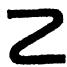
\includegraphics[keepaspectratio]{images/part003_0bad14cb.jpg}}

由命题 2 推出，有限个下半连续函数的下包络仍是下半连续的；但对无穷族下半连续函数的下包络，这一般不成立。例如，设 r 为任一有理数，\(f_{r}\) 表示在 r 处等于 0 而对一切实数 \(x \neq r\) 等于 1 的函数；诸 \(f_{r}\) 的下包络是函数 g，它对每个有理数等于 0，对每个无理数等于 1（``Dirichlet 函数''），而这个函数在无理点处不下半连续。

推论. 空间 X 上一族连续实值函数的上包络在 X 上下半连续。

在第九章，§ 1，第 6 节，命题 5 中我们将证明，若 X 是可一致化的（且仅在这种情形），这个命题的逆命题为真：可一致化空间上的每个下半连续函数是一族连续函数的上包络。

命题 3. 实值函数 \(f\) （定义在拓扑空间 \(\mathbf{X}\) 上）在一点 \(a \in \mathbf{X}\) 处下半连续，当且仅当 \(\liminf_{x \to a} f(x) = f(a)\) {[}或等价地，当且仅当 \(\liminf_{x \to a} f(x) \geqslant f(a)\) {]}。

该条件是必要的。因为对任意给定的 \(h < f(a)\) ，存在一个邻域 \(V\) （在 \(a\) 处），使得 \(h < f(x)\) 对一切 \(x \in V\) 成立；因此

\[
h \leqslant \inf _ {x \in \mathbf {V}} f (x) \leqslant \liminf _ {x \rightarrow a} f (x)
\]

（§ 5，第 6 节，公式 (12)），于是 \(f(a) \leqslant \liminf_{x \to a} f(x)\) 。该条件是充分的；因为若它成立，则对每个 \(h < f(a)\) 存在一个邻域 \(V\) （在 \(a\) 处），使得 \(h \leqslant \inf_{x \in V} f(x)\) ，从而 \(f\) 在 \(a\) 处下半连续。

命题 4. 设 \(f\) 是定义在子集 \(A\) （在拓扑空间 \(X\) 中稠密）上的任意实值函数。若对每个 \(x \in X\) 令 \(g(x) = \liminf_{y \to x, y \in A} f(y)\) ，则 \(g\) 在 \(X\) 上下半连续。

因为对任意给定的 \(h < g(x)\) ，存在一个开邻域 \(\mathbf{V}\) （在 \(x\) 处），使得对一切 \(z \in \mathbf{V} \cap \mathbf{A}\) 有 \(h < f(z)\) ；而 \(\mathbf{V}\) 是它的每个点 \(y\) 的邻域；于是 \(\liminf_{z \to y, z \in \mathbf{A}} f(z) = g(y) \geqslant h\) 对一切 \(y \in \mathbf{V}\) 成立，由此即得结果。

函数 g 称为 f 的下半连续正则化。~我们类似地定义 f 的上半连续正则化。

我们也可以把 \(g\) 定义为诸下半连续函数 \(\varphi\) （定义在 \(\mathbf{X}\) 上，且满足 \(\varphi(x) \leqslant f(x)\) 对一切 \(x \in \mathbf{A}\) 成立）中最大的一个。若 \(f\) 在 \(\mathbf{A}\) 上下半连续，则由命题 3，\(g\) 是 \(f\) 到 \(\mathbf{X}\) 的一个延拓。

